\chapter{Example - phytoplankton bloom}
Consider the ocean and its multitude of parameters that is possible to measure within it. Salt, plankton, herring abundance, pH, temperature, marine snow, speed of sound, density, vertical flux, light absorption and scattering, dissipation, currents, tides and waves to name a few. For each of these, adaptive sampling could be applied, in order to increase information gain. In doing so, the adaptive algorithm has to be better than deterministic sampling methods for the research question it is applied to. In this example, a noisy and dynamic phytoplankton bloom is attempted to be mapped with autonomous agents. In addition to providing the example, an attempt is made to present the research questions driving the design process and the alternatives present at any juncture. 



\section{Problem statement}
In this example, the following research questions will be explored. 
\begin{quote}
    \textbf{Question 1:} is it possible to make an adaptive sampling strategy for a phytoplankton bloom that is better than a deterministic one? 
\end{quote}

\begin{quote}
    \textbf{Question 2:} In a dynamic environment, is it possible to capture the variability in a meaningful way using adaptive sampling? 
\end{quote}

\section{Simulated chlorophyll field}
For this example, a simulated dynamic CF field is used, such that it can be interrogated for model accuracy. The simulated CF field was produced by choosing two (a and b) points and their corresponding radii, and calculating the value around those points in space and time. 
\begin{align}
        y_{sim} (x,y,d) &= \Bar{y} + 0.1 d e^{-0.1d} + 0.1\sigma_s  + c_{ma}\sigma_a \sigma_{az} +  c_{mb} \sigma_b \sigma_{bz} + \varepsilon_l \\
        \varepsilon_l &= y_{sim}^2 (e^{\varepsilon^2}-1) \\
        \varepsilon &\sim \mathcal{N}(0,\tau^2)
\end{align}


\begin{align}
    t_{tidal} &= 44700 \\
    x &= x + x_{tide}sin(2\pi (t + \Delta t_{x}) /t_{tidal})\\
    y &= y + y_{tide}sin(2\pi (t+ \Delta t_{y}) /t_{tidal})\\
    \sigma_a &= \frac{e^{(r_a-r_{aa})/f_t}}{e^{(r_a-r_{aa})/f_t}+1}\\
    \sigma_b &= \frac{e^{(r_b-r_{bb})/f_t}}{e^{(r_b-r_{bb})/f_t}+1}\\
    \sigma_{az} &= \frac{2e^{|d-d_a|}}{e^{3|d-d_a|}+1} \\
    \sigma_{bz} &= \frac{2e^{|d-d_b|}}{e^{3|d-d_b|}+1} \\ 
    \sigma_s &= \frac{e^{y/f_t}}{e^{y/f_t}+1}\\
    r_a &= \sqrt{(x-x_a)^2+(y-y_a)^2}\\
    r_b &= \sqrt{(x-x_b)^2+(y-y_b)^2}
\end{align}

With $x_{tide}$, $y_{tide}$, $\Delta t_{x}$, $\Delta t_{y}$, $\Bar{y}$, $x_a$, $x_b$, $y_a$, $y_b$, $d_a$, $d_b$, $r_{aa}$, $r_{bb}$, $f_t$, $c_{ma}$, and $c_{mb}$ as constants, allowing modification of the field, and $x$, $y$, and $d$ being the positional arguments with $d$ corresponding to depth. A realization of the field is plotted in Figure \ref{fig:appdx1}, using the constants as presented in Table \ref{tab:const_app}. 


\begin{figure}
    \centering
    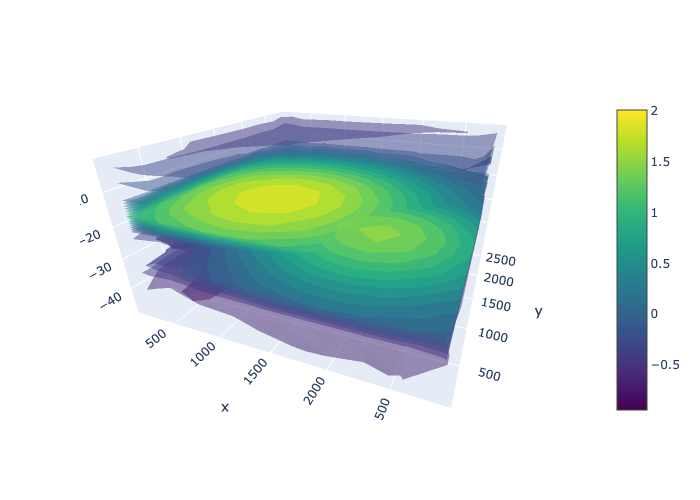
\includegraphics[width=0.8\textwidth]{figures/fig_gp_temp4.png}
    \caption{Simulated chlorophyll a fluorescence field, with no noise, $\tau = 0$, plotted on a $3000\text{m}\times3000\text{m}\times50$m operational volume used for simulation. Plotted using log-scale for easier visualization. }
    \label{fig:appdx1}
\end{figure}

\begin{figure}
    \centering
    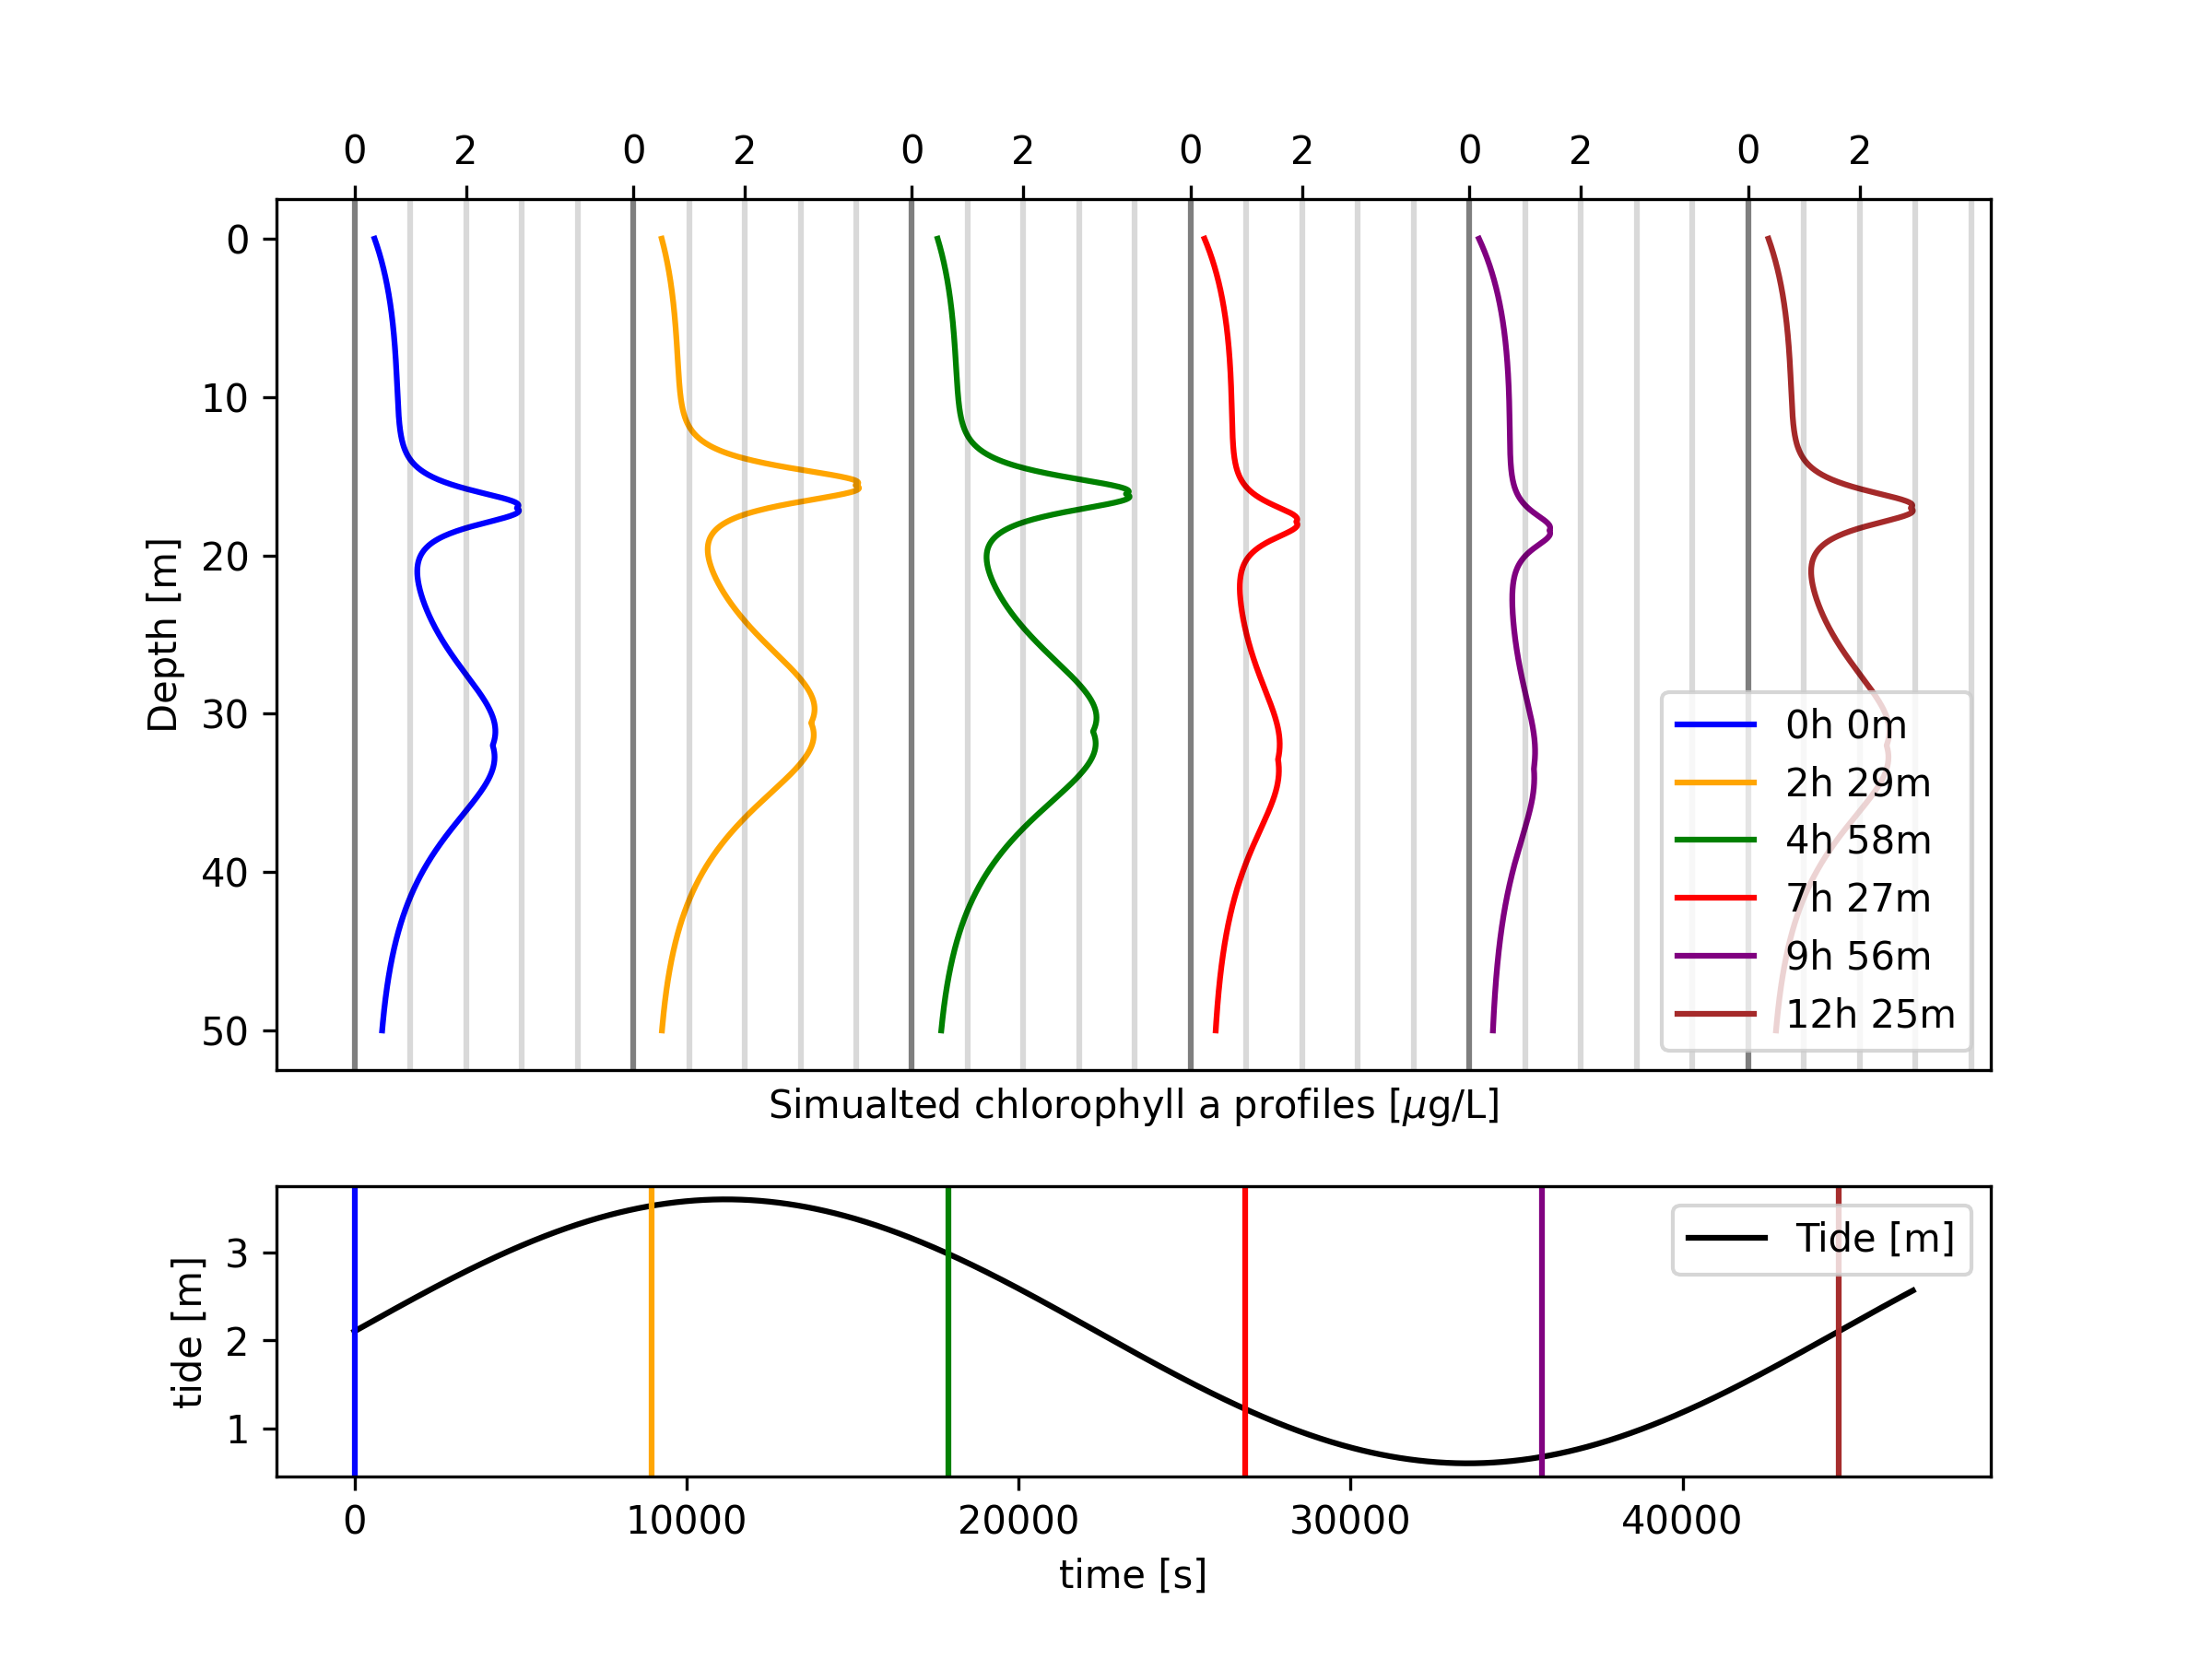
\includegraphics[width=0.95\textwidth]{figures/profilesx1350y150.png}
    \caption{Simulated chlorophyll-a fluorescence profiles at location $x=1350$m and $y=150$m, with no noise, $\tau = 0$, throughout the tidal cycle. }
    \label{fig:tidalsim}
\end{figure}


\begin{table}[]
    \centering
    \begin{tabular}{|c|c|c|c|c|c|c|c|}
    \hline
        $\Bar{y}$ & $x_a$ & $x_b$& $y_a$& $y_b$& $d_a$& $d_b$& $r_{aa}$  \\
        \hline
        0.3 & 1500 & 2500 & 1800 & 200 & 17 & 32 & 800 \\
        \hline 
        $r_{bb}$ & $f_t$& $c_{ma}$& $c_{mb}$ & $x_{tide}$ & $y_{tide}$ & $\Delta t_{x}$ &  $\Delta t_{y}$  \\
        \hline 
        700 & 400 & 8.0 & 5.5 & 1000 & 800 & 0 & 6705 \\
        \hline 
    \end{tabular}
    \caption{Chlorophyll a fluorescence simulator parameters used for simulation and testing. }
    \label{tab:const_app}
\end{table}


\subsection{Assumptions}
In designing an adaptive strategy for a fleet of autonomous agents, we need to make some assumptions about both the agents and the phenomena they set out to measure. The designer might review the literature, check the specifications and extrapolate from past experience, but none the less, they will need to make some assumptions. When applied to the problem at hand, the following assumptions were made: 
\begin{itemize}
    \item[\textbf{1:}] The AUV speed is greater than the process speed. 
    \item[\textbf{2:}] The distribution of measured chlorophyll a has a log-normal distribution. 
    \item[\textbf{3:}] 
\end{itemize}

Assumption \textbf{1} is reflecting the constraint of the AUV sampling envelope, as processes too fast for the AUV are not attempted to be measured. In the case of advection, the AUV would be advected with the water mass, potentially following the phenomena. Assumption \textbf{2} arises directly from the data, and the desire to model its distribution\cite{low2009multi,kemna2016adaptive,kemna2018multi}\textcolor{red}{PAPER 3 attempted this TODO}.  
\subsection{Physical drivers}
To better get a sense of what the robot is supposed to do, how the environment is expected to behave, we take a look at the physical drivers of a phytoplankton bloom. As spring arrives, so does the light, thhe transition from the dark to the light season is especially marked in the high latitudes. During the dark winter, nutrients have been mixed into the water column and the sun once again shines on the ocean, the phytoplankton bloom \cite{sakshaug2009ecosystem}. This reflects the two main physical drivers of the bloom: light and nutrients. The nutrients however, are quickly used up, and when they are, the bloom will occur in the deeper layers, gradually moving down. If there is a mixing event, such as a storm, the water column will homogenize, and a secondary bloom can occur near the surface. Additionally, strong stratification might trap phytoplankton in thin layers \cite{durham2012thin}. This is to say, that depending on weather, timing, and hydrographical conditions, the spatial distributions of phytoplankton may vary exstensibly. 

\subsection{Biological drivers}
All organisms strive for survival, this includes the grazers, a class of plankton that eat phytoplankton, reducing their stock. These grazers are then eaten by other plankton, fish, jellies, and larvae, making their impact on the phytoplankton stock at unpredictable at any time.  

Thus, with both physical and biological drivers contribute to the spatial distributions of phytoplankton being highly heterogeneous \cite{grunbaum2012logic}. 



\section{Method choice}
In choosing a method for adaptive sampling of the marine phytoplankton bloom, we must take the scientific objective into account. For this, \textbf{research question 1} is investigated: "is it possible to make an adaptive sampling strategy for a phytoplankton bloom that is better than a deterministic one? " From the literature \cite{frolov2014can}, we know that, yes, it is possible.

However, what is meant by \textit{better}? From an information theoretic standpoint that might be a smaller posterior error or uncertainty. From an oceanographic standpoint it might mean that the target phenomenon was studied without much time spent searching for it. What we might choose to define as the goal of the sampling will inform what is better and what is worse. 

\subsection{Comparison criterion}
In order to compare different modes of modelling and behavior, a metric for comparison is needed. No only for this example, but for the operator developing and testing a new method. Benchmarking against other methods is not usually done in adaptive sampling, but it is encouraged by the author. In choosing a criterion for bencmharking, the optimization criterion is also implicitly chosen for the adaptive methods. In this case, it is possible to compare the \acrshort{rmse} of different the predictive mean of different modelling and sampling strategies. 

\subsection{Subsumption-based method alternatives}
As the CF field can have a multitude of shapes and amplitudes, a general, rule-based approach can be hard to formulate. It has, however, been attempted\cite{fossum2019toward} in the vertical plane. This was done by modelling the depth of the \acrfull{scm} as a two-dimensional \acrshort{gp}, similar to the river plume depth estimation in \textbf{paper B}. Another subsumption-based attempt at following the \acrshort{scm} \cite{zhang2019autonomous} found the isotherm associated with it and used the temperature as a feedback for depth control, and running the \acrshort{auv} in tight circles for it to act as a pseudo-Lagrangian drifter. 

\subsection{Measurements}
Measurements made of a phytoplankton blooms with fluorometers tend to be log-normally distributed\cite{low2009multi,kemna2016adaptive}, and noisy as discussed in \textbf{paper C}. Fluorometers noise tend to be driven both by measurement noise from a low signal to noise ratio, and \textit{process noise}, arising from measuring a small sampling volume ($\simeq 3$ml\cite{boss2016primer}) in relation to the movement speed and sampling frequency. Add to this that phytoplankton patches can have cm-resolutions\cite{mitchell2008phytoplankton,durham2012thin}, sampling frequencies are between 1 and 2 Hz, as in \textbf{paper C}, and the \textit{process noise} can be interpreted as a collection of structures outside the sensor capabilities. Keeping this in mind, filtering and estimating the measurement noise becomes important, as it was for the gradients captured in \textbf{papers A} and \textbf{B}. 


\section{GP implementation}
In this example, the $\ell$\acrshort{gp} formulation from \textbf{paper C} is followed, creating a three dimensional model, with temporally increasing uncertainty on the measurements. As the model has to be used for on-board decision making, the number of grid points is set purposefully low. 

\subsection{Formulation}
 Denoting a set of measurements $\mathbf{y}_{S}$ at locations $X$ at times $\mathbf{\tau}$, with $S = [X,\mathbf{\tau}]$ and let $\mathbf{z}_{S} = log_e \mathbf{y}_{S} - \mathbf{m}_{GP}$, where $\mathbf{m}_{GP} = \overline{log_e \mathbf{y}_{S}}$ is the mean of the input data. In taking the logarithm of the measurements, they become unit-less \cite{matta2011can}. Assuming that $\mathbf{z}_{S} \sim \mathcal{N}(\mu,\sigma_c^2) $, such that a GP could be used for predictions of $\mathbf{z}$ at unobserved locations and times by the formulation in equations \eqref{eq:gp_1} to \eqref{eq:gp_3}\cite{rasmussen2003gaussian}.

\begin{align}
    \label{eq:gp_1}
    & \mathbf{f}_*|S,\mathbf{z}_S,S_* \sim \mathcal{N}(\Bar{\mathbf{f}}_*,cov(\mathbf{f}_*))\text{, where} \\
    \label{eq:gp_2}
    & \Bar{\mathbf{f}}_* \triangleq \mathbb{E}[\mathbf{f}_*|S,\mathbf{z}_S,S_*] =  K_{S_*,S}[K_{S,S}+\sigma_n^2 I]^{-1}\mathbf{z_s} + \mathbf{m}_{GP} \\
    \label{eq:gp_3}
    & cov(\mathbf{f}_*) = K_{S_*,S_*} - K_{S_*,S}[K_{S,S}+\sigma_n^2 I]^{-1}K_{S,S_*}
\end{align}

\subsection{Model parameters}
In order to initiate the model, some prior knowledge is required, not only about the current conditions, but also of the statistical properties of the field. While the variance, nugget and de-correlation lengths can be learned on-line, they are often set beforehand, as in \textbf{papers B, C, F, and G}, and in the literature \cite{kemna2016adaptive,kemna2018multi,fossum2019toward,fossum2018information}. In this case, the horizontal length scale for the field is set to $600$m, in both x- and y-direction, making the horizontal plane isotropic. The length scale in z-direction has to be set much smaller, at $3$m, due to the oceans \textit{stratification} or flatness. 


\subsection{Temporal effects}
Depending on the expected duration of the mission, it is possible to add temporal effects, such as adding temporally increasing noise to old measurements (\textbf{paper C}), or to try to model the currents and advection \cite{berget2022adaptive}. In this case, temporally increasing noise will be added, by adding a term in the kernel, the de-correlation time. 

\subsection{Kernel}
The choice of kernel can depend on a multitude of factors, but mainly the data available. In this case, the underlying simulation model is available, making it possible to construct a semivariogram for the choice of kernel and parameters. 

\section{Path planning}
HAs to be done along the model selection, at this point it becomes a challenge
\subsection{potential paths}
\subsection{utility function}
\subsection{one-step-aheadf}
Yaolins method

\section{Performance}
\subsection{Posterior map error}
\subsection{Scientific value (?)}
\subsection{..}

